\chapter{O Modelo Implementado}

Para implementar o ambiente de teste de \emph{cloud computing},
foi escolhida a pilha de ferramentas conhecida
como \emph{OpenStack}, implementada usando um nó para controle e \emph{networking}
da nuvem e outro nó para processamento. O modelo de rede escolhido para o ambiente
de testes foi o que é chamado pelo \emph{OpenStack} de \emph{simple flat networking},
onde apenas uma interface de rede é utilizada para todas as comunicações entre os serviços.
A instalação foi concebida com auxílio de
uma ferramenta de automação fornecida pela \emph{Rackpsace}, uma das empresas
criadores do próprio \emph{OpenStack} e uma das maiores do ramo de hospedagem
baseada em \emph{cloud computing}. Inicialmente, a intenção é de uma
nuvem privada, somente para uso interno da universidade. É esperada
uma evolução do projeto para uma nuvem híbrida, englobando também o conceito
de uma nuvem pública, para oferecer para empresas e outras insituições da região
os benefícios do \emph{cloud computing}.

\section{OpenStack}

O \emph{OpenStack} é um grupo de ferramentas, comumente chamado de ``ecossistema''
por sua comunidade desenvolvedora e utilizadora. Esse grupo é composto por
diversos serviços, são eles:

\begin{itemize}
    \item
        Keystone: serviço de autenticação entre os nós e serviços;

    \item
        Nova: serviço de processamento, que é responsável por distribuir,
        configurar e executar máquinas virtuais propriamente ditas;

    \item
        Glance: serviço responsável pela descoberta, registro e fornecimento
        de imagens de máquinas virtuais;

    \item
        Swift: serviço de armazenamento de objetos (arquivos), semelhante
        ao \emph{Amazon Simple Storage Service} (S3);

    \item
        Cinder: serviço de armazenamento de blocos, responsável por armazenar
        os discos virtuais utilizados pelas máquinas virtuais;

    \item
        Neutron: serviço de gerenciamento de redes virtuais, responsável
        por simular switches e roteadores e atribuir IPs às máquinas
        virtuais;

    \item
        Horizon: serviço de gerenciamento da nuvem. Fornece uma interface
        web para controle de tudo o que os outros serviços fornecem.
\end{itemize}

Pode-se observa como cada parte se comporta e com quem se comunica dentro do sistema
através da Figura \ref{img:openstack-services}.

\begin{figure}[h]
  \center
  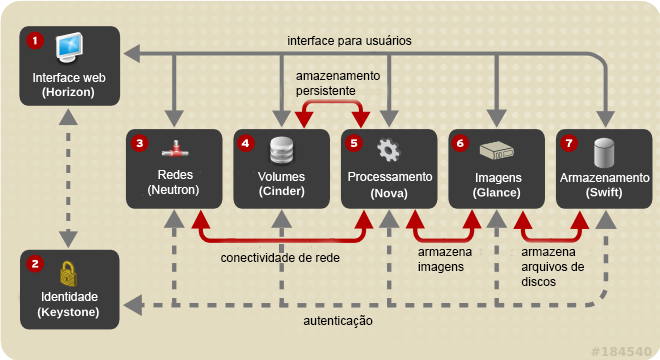
\includegraphics[scale=1.0]{imagem/openstack-services.png}
  \caption{Arquitetura do OpenStack}
  \caption*{Fonte: \url{https://access.redhat.com/documentation/en-US/Red_Hat_Enterprise_Linux_OpenStack_Platform/2/html/Getting_Started_Guide/ch01.html}}
  \label{img:openstack-services}
\end{figure}

Segundo \citeonline{rackspace-nasa-openstack}, este ecossistema foi fundado pela NASA e
pela \emph{Rackspace Hosting} e a partir de então teve uma grande adesão de
parceiros, tanto no meio científico quanto no meio corporativo. Um destes
grandes parceiros na área científica é o \emph{CERN} (Organização Europeia
para Pesquisa Nuclear), que analisa dados coletados pelo famoso \emph{LHC}
(Grande Colisor de Hádrons). \citeonline{cern-openstack} diz que
o \emph{OpenStack} é de grande importância dentro desta organização, fornecendo
recursos computacionais em larga escala para físicos espalhados pelo globo com
menos gargalos burocráticos.

Estes fatores, aliados às contribuições de diversos membros da comunidade de
software livre para uma rápida evolução do ecossistema foram essenciais para a
escolha destas ferramentas. Hoje, o projeto conta com novas versões a cada 6
meses, sempre incoporando diversas funcionalidades e implementando sugestões
de diversos usuários. A fundação do \emph{OpenStack} é composta por um comitê
técnico de 13 membros eleitos por contribuidores tecnológicos, um quadro de
24 diretores, sendo 8 apontados por membros, 8 eleitos por membros de classe e
8 eleitos por membros comuns, e por um comitê de usuários composto por mais de
75 grupos espalhados por todo o mundo.

\subsection{História}

Em 2008, os esforços da NASA para padronizar seus \emph{websites} inspiraram
uma explosão em tecnologias de \emph{cloud computing} \cite{nasa-cloud-computing}.
O projeto, em seu início, era chamado de \emph{NASA.net} e tinha como objetivo
unificar todas abordagens usadas para desenvolver tais \emph{websites}. Todos eles
pareciam diferentes e eram gerenciados de maneiras diversas. A idéia era
que os desenvolvedores pudessem criar seus \emph{websites}, enviá-los para o
\emph{website} do \emph{NASA.net} e ele tomaria conta de todos os passos necessários.

Apesar que o projeto estava apenas começando naquela época, seus desenvolvedores
já identificaram a necessidade de ter grandes ferramentas na sua fundação. O próximo
passo era construir um ``serviço de infraestrutura''. Foi criada então uma plataforma
capaz de fornecer poder computacional para rodar serviços da \emph{NASA.net} e que
também poderia ser usado para outros tipos de aplicações. O que a equipe de desevolvimento
percebeu foi que eles precisavam desenvolver um serviço de \emph{cloud computing}.
A idéia era se autenticar no serviço e dizer: preciso de 10 computadores e,
dentro de um minuto, ter acesso a estes 10 computadores para qualquer que seja
o propósito.

Conforme o escopo do projeto cresceu, ele foi renomeado para \emph{Nebula}. O \emph{Nebula}
estava fazendo muitos mais do que criar padrões para os desenvolvedores \emph{web}
da agência: era fornecida uma grande gama de serviços para desenvolvedores, pesquisadores,
e cientistas, para que eles pudessem acessar e gerenciar toda enorme quantidade de
dados que a NASA acumulava dia após dia.

Um dos pontos decisivos sobre o sucesso do \emph{Nebula}, antes de se tornar
oficialmente \emph{OpenStack} foi a escolha do modelo de \emph{software} livre.
\emph{Software} proprietário é tão útil e conveniente algumas vezes que a equipe
chegou a pensar se seria possível continuar o desenvolvimento do produto sem se
apoiar neste modelo. Por outro lado, o modelo de desenvolvimetno de código aberto facilitaria
um ambiente colaborativo: qualquer um com o conhecimento poderia melhorar o código. Esta
foi então a escolha, segundo O'Brien (um dos criadores e idealizadores da ferramenta),
desde o início era desejado que o projeto envolvesse uma grande comunidade (empresas
privadas, instituições acadêmicas e laboratórios de pesquisa, por exemplo) que
pudesse contribuir e levar o \emph{Nebula} a um nível mais alto.
O \emph{Nebula} acabou por evoluir e se tornar um projeto que estava atendendo
demandas e necessidades gerais, não somente da NASA, mas do mundo todo. Entretanto,
houve um problema com umas das partes do sistema, feita com software proprietário,
que precisava ser migrada para uma linguagem aberta. A linguagem escolhida foi Python, a
preferida da equipe de desenvolvimento.

A partir da publicação do \emph{Nebula} como \emph{software} livre, foi chamada
a atenção de diversos membros da indústria. Um deles, uma empresa de hospedagem
conhecida como \emph{Rackspace}, que também desenvolvia suas próprias
ferramentas para automatizar o processo de gerenciamento das aplicações
que seus clientes queriam hospedar, estava pronta para liberar suas próprias
ferramentas dentro do mesmo modelo de código aberto. Com a notícia, a Rackspace,
que tinha paixão por \emph{software} livre, entrou em contato com a equipe do \emph{Nebula}
para colaborar com o desenvolvimento do projeto. Um complementou o outro, e da
fusão dos dois projetos foi anunciado o \emph{OpenStack}, atraindo milhares de
colaboradores por todo o mundo e centenas de grandes empresas. Antes, o que
somente poderia ser feito pagamento para um terceiro, poderia ser então
feito de maneira totalmente gratuita, com uma ferramenta gratuita e aberta.

\subsection{Modelo de rede}

Uma das características mais complexas do ecossistema escolhido é a arquitetura
de rede. O ambiente de produção ideal deve fornecer 4 interfaces de rede para
total separação dos tráficos de gerenciamento, dos sistemas de armazenamento,
da rede privada das máquinas virtuais e da rede pública (que fornece IPs
flutuantes) e assim atingir o máximo de performance.

De acordo com a documentação do \emph{OpenStack}, é possível usar no mínimo duas interfaces de rede
com um \emph{switch} gerenciável, ou seja, capaz de roteamento de pacotes nas camadas 2 e 3
do modelo OSI, através de uma técnica conhecida como \emph{VLAN tagging} (\cite{l2-l3-vlan}). Também pode-se
chegar ao caso mais básico e simples: uma única interface de rede,
com o uso de um um nó de \emph{networking} (usando a ferramenta \emph{Neutron})
para desempenhar este papel, porém usando uma técnica conhecida como \emph{GRE} (Generic
Routing Encapsulation), que tem como desvantagem uma certa lentidão
para o encapsulamento dos pacotes e gera um gargalo na inteface de rede deste
nó (todo tráfego precisa passar por ele).

Para este ambiente de testes, logicamente, foi usado o modelo de rede mais
simples, conhecido como \emph{simple flat networking}, dada a facilidade
de implementação deste utilizando a ferramenta Neutron e a técnica \emph{GRE}.

\subsection{Configuração e instalação}

Foram realizadas diversas tentativas de instalação e configuração do projeto
utilizando os manuais do próprio \emph{OpenStack}, disponíveis na documentação
oficial, porém sem sucesso. São diversas configurações espalhadas por arquivos
diferentes e diversos comandos extremamente sensíveis. Se um erro é cometido,
ele só será notado quando todas as ferramentas do ecossistemas forem instaladas
e implicará em uma análise de \emph{logs} para futura correção. Como solução
para este problema, o próprio projeto recomenda o uso de ferramentas de automação,
sendo as mais conhecidas: \emph{Salt}, \emph{Puppet} e \emph{Chef}.

Para o desenvolvimento deste ambientes de testes, foi escolhida a ferramenta
\emph{Chef}, usada com scripts fornecidos pela própria Rackspace, por causa
do excepcional suporte oferecido pela empresa, tanto para o seu uso quanto para
toda a configuração necessária, através do programa \emph{Rackspace Private Cloud}.
Durante todo o processo (que será descrito abaixo), diversos problemas na ferramenta de automação
fornecida pela Rackspace foram encontrados e reportados à equipe de desenvolvimento,
que rapidamente corrigiu-os para que fosse possível continuar o procedimento.
O programa \emph{Rackspace Private Cloud} compreende um pacote de \emph{software livre} para a instalação do
\emph{OpenStack}, treinamento e certificação, prestação de serviços e opções
de suporte para auxiliar a construção e gerenciamento da nuvem privada. Como
eles possuem a maior infraestrutura baseada no \emph{OpenStack} do mundo, há possibilidade
de acesso aos profissionais que participaram deste grande feito e enfrentaram os
mais diversos problemas para tal infraestrutura.

O \emph{Chef} é uma ferramenta de automação e gerenciamento de infraestrutura
baseada no modelo cliente-servidor. Tarefas para controle de infraestrutura,
chamadas de de \emph{recipes} (receitas), definem instruções
para instalar e configurar bancos de dados, servidores web e balanceadores de
carga, por exemplo. Estas receitas, por sua vez, são compostas de \emph{resources}
(recursos), como um arquivo, um \emph{template} ou um pacote do sistema a ser instalado.
Há também a possibilidade de agrupar receitas em \emph{roles}, ou papéis, para
uma maior abstração da infraesturura, permitindo que diversas receitas sejam
executadas em múltiplos nós. Todas as receitas e papéis são armazenados no servidor
(\emph{chef-server}) e os clientes se registram e sincronizam-se através do
\emph{chef-client}. A partir deste ponto, ao comando do servidor, os próprios
clientes executam as receitas das dos papéis atribuitdos a eles em si mesmos. Para
configuração tanto do chef-server quando dos nós que serão provisionados através
do \emph{chef-client}, existe a ferramenta \emph{knife}. Ela que envia o \emph{cookbook}
(conjunto de receitas) para o chef-server e faz o registro dos \emph{chef-clients}
neste servidor. Tal ferramenta pode ser instala no próprio \emph{chef-server} ou em
outro computador, conforme necessidade e conveniência. Veja a Figura \ref{img:chef}
para uma melhor compreensão da organização e comunicação deste conjunto.

\begin{figure}[h]
  \center
  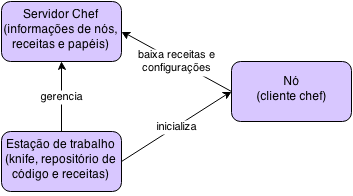
\includegraphics[scale=1.0]{imagem/chef.png}
  \caption{Fluxograma de funcionamento do Chef}
  \label{img:chef}
\end{figure}

Finalizando, para o ambiente de testes foram utilizados 4 computadores
e um pequeno roteador, cedidos pelo Laboratório Ada Lovelace, do curso de
Ciência da Computação da UENF. Cada um dos computadores possui a seguinte configuração:

\begin{itemize}
    \item Processador: Core i5 de segunda geração, com 4 núcleos rodando a 3.4 Ghz;
    \item Memória: 4GB DDR3 1066 Mhz;
    \item Disco rígido: HDD 160GB 7200rpm.
    \item Sistema Operacional: Ubuntu Server 12.04 64 bits
\end{itemize}

Um deles foi configurado para ser o \emph{chef-server}, um para ser o nó controlador
da nuvem e um nó para processamento das máquinas virtuais. Basicamente, o processo de
instalação consiste nos seguintes passos:

\begin{enumerate}
  \item Preparação do nós (instalação de sistema operacional)
  \item Instalação do \emph{chef-server}, dos livros de receitas da Rackspace
  \item Criação de um ambiente \emph{chef} e definição dos seus atributos (configurações)
  \item Instalação do \emph{chef-client} nos nós
  \item Atribuição e aplicação dos papéis aos nós controlador, de rede e de
    processamento
\end{enumerate}

Como a preparação dos nós é aberta para ser feita de acordo com o costume do usuário,
bastando que seja instalado o sistema operacional indicado, este passo não será
descrito.

\subsubsection{Instalação do chef-server e livros de receitas
da Rackspace}

Após preparar os nós, escolhe-se um para ser o \emph{chef-server} e então,
logado como o usuário \emph{root}, instala-se o software com os comandos mostrados
no Código \ref{cod:chef-server-install}

\begin{listing}
\begin{minted}[frame=lines,framerule=2pt]{bash}
  $ curl -s -O https://raw.githubusercontent.com/rcbops/support-tools/
  master/chef-install/install-chef-server.sh
  $ bash install-chef-server.sh
\end{minted}
\caption{Instalação do \emph{chef-server}}
\label{cod:chef-server-install}
\end{listing}

Após este processo terminar, recarrega-se o terminal para atualizar as variáveis
necessárias e testa-se o comando \emph{knife} através dos comando no Código \ref{cod:test-chef}.

\begin{listing}
\begin{minted}[frame=lines,framerule=2pt]{bash}
  $ source /root/.bash_profile
  $ knife client list
\end{minted}
\caption{Teste de instalação do \emph{chef}}
\label{cod:test-chef}
\end{listing}

A instalação dos livros da receitas da Rackspace é feita através dos seus repositórios
de código, seguindo os comandos do Código \ref{cod:chef-cookbooks}.

\begin{listing}
\begin{minted}[frame=lines,framerule=2pt]{bash}
  $ git clone https://github.com/rcbops/chef-cookbooks.git
  $ cd chef-cookbooks
  $ git checkout 4.1.2
  $ git submodule sync
  $ git submodule update
  $ knife cookbook upload -a -o cookbooks
  $ knife role from file roles/*rb
\end{minted}
\caption{Instalação dos livros de receitas da Rackspace}
\label{cod:chef-cookbooks}
\end{listing}

\subsubsection{Criação do ambiente para configuração do OpenStack}

A partir dai é iniciada a parte de criação do ambiente no \emph{chef} e
configuração das variáveis do \emph{OpenStack} em si. Para criar o ambiente e
abrir o arquivo de configuração, executa-se os comandos apresentados no Código
\ref{cod:knife}.

\begin{listing}
\begin{minted}[frame=lines,framerule=2pt]{bash}
  $ knife environment create private-cloud -d "UENF Private Cloud"
  $ knife environment edit private-cloud
\end{minted}
\caption{Criação do ambiente do \emph{chef}, visualização e edição das variáveis
 deste ambiente}
\label{cod:knife}
\end{listing}

Ao executar o último comando, será aberto o arquivo em branco, onde deve-se
sobrescrever as variáveis padrões definidas pela Rackspace de maneira
adequada à infraestrutura onde o sistema está sendo configurado. Como mencionado
anteriormente, o modelo de rede é complicado, tomando um tempo considerável para
sua compreensão e o fato de haver somente uma interface de rede para o ambiente
de testes adicionou uma complexidade extra ao processo. A equipe de suporte
da Rackspace teve que ser acionada para auxiliar o processo de configuração.
A partir dai, o arquivo de configuração ideal para a implantação do ambiente
de teste foi estabalecido como mostrado no Código \ref{cod:json}. Nesta imagem
pode-se observar no atributo \emph{osop\_networks} que as 3 redes utilizadas
pelo \emph{OpenStack} estão configuradoas sob a mesma faixa de IPs, ou seja,
todas elas na mesma interface de rede.

\begin{listing}
\begin{minted}[frame=lines,framerule=2pt]{javascript}
{
  "name": "rpcv412",
  "description": "Rackspace Private Cloud v4.2.2",
  "cookbook_versions": {
  },
  "json_class": "Chef::Environment",
  "chef_type": "environment",
  "default_attributes": {
  },
  "override_attributes": {
    "nova": {
      "libvirt": {
        "vncserver_listen": "0.0.0.0"
      },
      "network": {
        "provider": "neutron"
      }
    },
    "neutron": {
      "ovs": {
        "provider_networks": [
          {
            "label": "ph-eth0",
            "bridge": "br-eth0",
            "vlans": "1:1"
          }
        ],
        "network_type": "gre"
      }
    },
    "mysql": {
      "allow_remote_root": true,
      "root_network_acl": "%"
    },
    "osops_networks": {
      "nova": "192.168.0.0/24",
      "public": "192.168.0.0/24",
      "management": "192.168.0.0/24"
    }
  }
}
\end{minted}
\caption{Arquivo de configuração das variáveis utilizadas para o ambiente de testes
montado}
\label{cod:json}
\end{listing}

\subsubsection{Instalação do chef-client nos nós da cloud}

Para a configuração do \emph{chef-client} nos nós onde os componentes do \emph{OpenStack}
serão instalados, é necessária a criação de uma chave SSH para conexão sem senhas e depois
proceder a instalação usando a ferramenta \emph{knife bootstrap}, como visto no Código
\ref{cod:knife-bootstrap}, substituindo \emph{\textless usuario\textgreater} e
\emph{\textless ip\textgreater} pelo usuário e IP
de cada nó que se deseja adicionar ao ambiente.

\begin{listing}
\begin{minted}[frame=lines,framerule=2pt]{bash}
$ ssh-keygen
$ knife bootstrap -E private-cloud -i .ssh/id_rsa_private --sudo
-x <usuario> <ip>
\end{minted}
\caption{Código para realizar a configuração do \emph{chef-client} nos nós do ambiente}
\label{cod:knife-bootstrap}
\end{listing}

Após o processo terminar, é necessário que cada nó da rede possa acessar o
\emph{chef-server} pelo \emph{hostname}. Para isto, adiciona-se uma linha
para cada nó no arquivo \emph{/etc/hosts} seguindo o seguinte modelo do Código
\ref{cod:hosts}. A partir daí, o registro do nó cliente com o \emph{chef-server} é feito
executando-se comando \emph{chef-client}.

\begin{listing}
\begin{minted}[frame=lines,framerule=2pt]{text}
<ip-chef-server> <hostname-chef-server>
\end{minted}
\caption{Modelo de arquivo de configuração de \emph{hosts} nos nós clientes}
\label{cod:hosts}
\end{listing}

\subsubsection{Atribuição e aplicação dos papéis aos nós}

Prossegue-se então com a atribuição dos papéis aos nós que farão parte da
\emph{cloud}. Como dito anteriormente, para o ambiente de teste foram usados
um nó controlador, um de rede e um de processamento. São executados os comandos
mostrados no Código \ref{cod:role} em cada nó, substituindo o \emph{\textless papel\textgreater}
por \emph{role[ha-controller]}, \emph{role[single-compute]} e \emph{role[single-network]}
e \emph{\textless hostname\textgreater} pelo \emph{hostname} deste mesmo nó.

Ao fim do procedimento, o \emph{OpenStack} já deve estar acesível através do
painel Horizon através do IP do nó controlador. A autentição pode ser feita
com o usuário \emph{admin} e a senha \emph{secrete}. Estas credenciais podem
ser modificadas a qualquer momento e outras mais também podem ser criadas.

Pode-se adicionar mais nós de rede e processamento de máquinas virtuais
conforme necessário, repetindo os processos de preparação do nó a ser adicionado,
instalação do \emph{chef-client} (Código \ref{cod:knife-bootstrap}),
configuração do arquivo de \emph{hosts} (Código \ref{cod:hosts}), atribuição
do papel (Código \ref{cod:role}) e execução do comando \emph{chef-client} no
próprio nó.

\begin{listing}
\begin{minted}[frame=lines,framerule=2pt]{bash}
$ knife node run_list add <hostname> '<papel>'
\end{minted}
\caption{Comando para atribuit um papel a um nó}
\label{cod:role}
\end{listing}
